\documentclass[12pt]{article}
\usepackage[utf8]{inputenc}
\usepackage[left=2.5cm, right=2.5cm, top=2.0cm]{geometry}
\usepackage{sectsty}
\usepackage{graphicx}
\usepackage{amsmath}
\usepackage{amssymb}
\usepackage{undertilde}
\usepackage{kbordermatrix}
\usepackage{listings}
\usepackage{ulem}
\usepackage{soul}
% \usepackage{tikz}
% \usepackage{pgfplots}
% \pgfplotsset{compat=1.16} 
\usepackage{siunitx}
\usepackage{pythonhighlight}
\usepackage{caption}
\usepackage{float}
\usepackage{url}
\usepackage{enumitem}
\usepackage{bm}
\usepackage{empheq}
\usepackage{tcolorbox}
\usepackage{framed}
\usepackage{xparse}
\usepackage{algorithm, algorithmic}
% \usepackage{algorithmic}
\usepackage{booktabs}
\usepackage{tabularx}
% ref packages
\usepackage{nameref}
% folowing  must be in this order
\usepackage{varioref}
\usepackage{hyperref}
\usepackage{cleveref}
\usepackage{mathtools}
\DeclareMathOperator*{\argmax}{arg\,max}
% \usepackage[shortlabels]{enumitem}
\tcbuselibrary{breakable}
\allowdisplaybreaks


%  ---------------------- COMMANDS ---------------------------
% Double underline
\def\dunderline#1{\underline{\underline{#1}}}

% Shorten nonumber command
\def\nnb{\nonumber}

% Shorten boldsymbol command
\def\bs#1{\boldsymbol{#1}}

% Algorithmic newline
\def\algonewline{\STATE{ }}

% Eigenvectors of
\def\eigvecof{\text{eigenvectors of }}

% Eigenvalues of 
\def\eigvalof{\text{eigenvalues of }}

% Enclose in square brackets
\newcommand{\enclb}[1]{\left[#1\right]}
% Enclose in parenthesis
\newcommand{\enclp}[1]{\left(#1\right)}
% Enclose in curly brackets
\newcommand{\enclc}[1]{\left\{#1\right\}}

% Annotate first argument, text in second argument
\newcommand{\overtext}[2]{\overbrace{#1}^{\mathclap{\text{#2}}}}
\newcommand{\undertext}[2]{\underbrace{#1}_{\mathclap{\text{#2}}}}

% Normalization constant in multivariate normal
\newcommand{\mvnconst}[1]{\frac{1}{(2\pi)^{d/2} |#1|^{1/2}}}

% Exponential factor in multivariate normal
\newcommand{\mvnexpo}[3][x]{\exp \left[  -{\frac{1}{2}} (#1 - #2)^T #3^{-1} (#1 - #2) \right]}

% Multivariate normal
\newcommand{\mvn}[3][x]{\mvnconst{#3} \mvnexpo[#1]{#2}{#3}}

% For numbering in align* environment
\newcommand{\numberthis}{\addtocounter{equation}{1}\tag{\theequation}}

%  Sum notation w/ limits as argument and index as option
\newcommand{\sumlim}[3][i]{\sum\limits_{#1=#2}^{#3}}

%  Product notation w/ limits as argument and index as option
\newcommand{\prodlim}[3][i]{\prod\limits_{#1=#2}^{#3}}

%  Sum notation with only information beneath
\newcommand{\sumnolim}[1]{\sum\limits_{#1}}

%  Integral notation w/ limits as argument and index as option
\newcommand{\intlim}[2]{\int\limits_{#1}^{#2}}

%  Integral over whole domain notation, no args
\newcommand{\intinf}{\int\limits_{-\infty}^{\infty}}

%  Partial derivative notation, arg1: numerator, arg2: denominator
\newcommand{\pfrac}[3][ ]{\frac{\partial^{#1} #2}{\partial #3^{#1}}}

%  Derivative notation, arg1: numerator, arg2: denominator
\newcommand{\dvfrac}[3][ ]{\frac{\text{d}^{#1} #2}{\text{d} #3^{#1}}}

% When doing Gauss-Jordan, create arrow showing operations
\newcommand{\ro}[1]{\xrightarrow{\mathmakebox[\rowidth]{#1}}}

% ----------------------INVIRONMENTS---------------------------
% Item list with title
\newenvironment{titlemize}[1]{%
  \paragraph{#1}
  \begin{itemize}}
  {\end{itemize}}

  % Enum list with title
\newenvironment{titleenum}[1]{%
  \paragraph{#1}
  \begin{enumerate}}
  {\end{enumerate}}

  % Augmented matrix (matrix with vertical line)
\newenvironment{sysmatrix}[1]
  {\left(\begin{array}{@{}#1@{}}}
  {\end{array}\right)}

 % Make matrices with more spacing
\makeatletter
\renewcommand*\env@matrix[1][\arraystretch]{%
  \edef\arraystretch{#1}%
  \hskip -\arraycolsep
  \let\@ifnextchar\new@ifnextchar
  \array{*\c@MaxMatrixCols c}}
\makeatother

% \renewcommand*{\arraystretch}{1.5}

\newlength{\rowidth}% row operation width
\AtBeginDocument{\setlength{\rowidth}{3em}}

\floatname{algorithm}{Algorithm}
\renewcommand{\algorithmicrequire}{\textbf{Input:}}
\renewcommand{\algorithmicensure}{\textbf{Output:}}

\begin{document}
\title{\textbf{INF367A Project 1}}
\author{Naphat Amundsen}
\maketitle
\sectionfont{\fontsize{14}{15}\selectfont}
\subsectionfont{\fontsize{12}{15}\selectfont}
\subsubsectionfont{\fontsize{12}{15}\selectfont}
\graphicspath{ {./images/} }

\ifx
\begin{figure}[H]
	\centering
	\includegraphics[scale=0.8]{Figure_2}
	\caption{Insert caption here}
\end{figure}
\fi
\ifx
\begin{figure}[H]
	\centering
	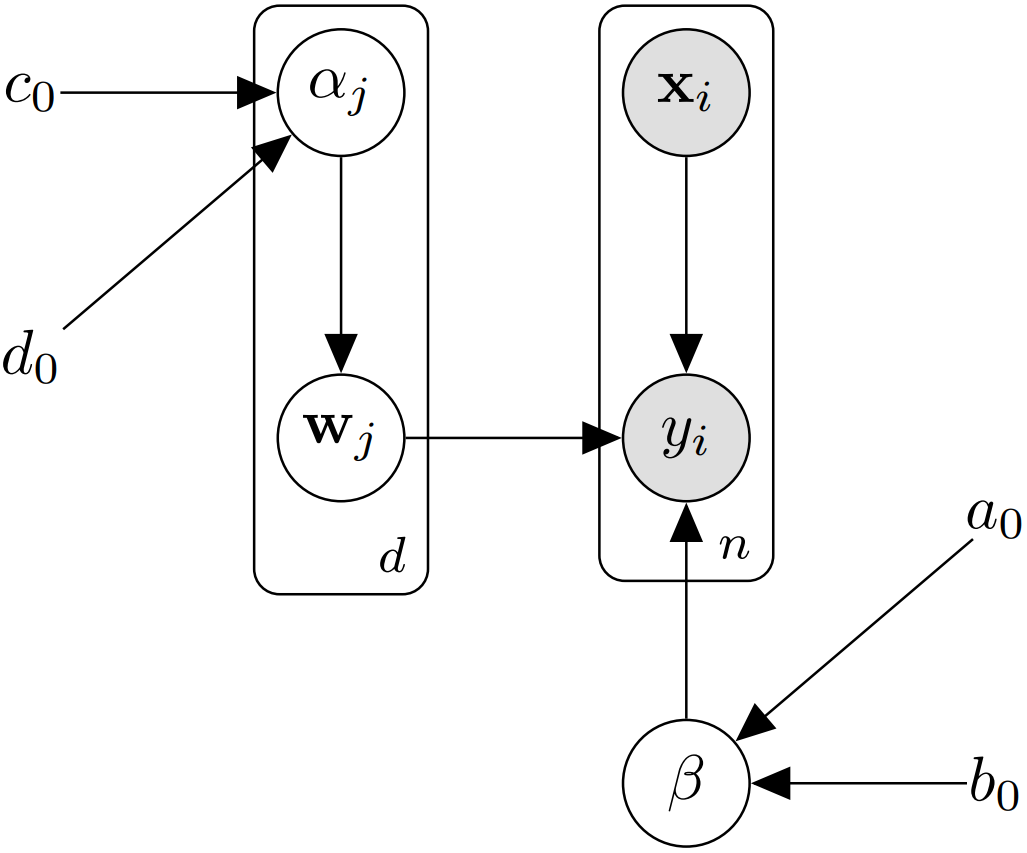
\includegraphics[scale=0.8]{bn_network.png}
	\caption{Plate diagram of the regression model with ARD prior. Variables $x_i$ , and $y_i$ are observed; We are interested in the posterior distribution of parameters $w$, $\alpha$ and $\beta$. The constants $a_0$ , $b_0$, $c_0$ , and $d_0$ are user-defined hyperparameters}
\end{figure}
\fi

\newcommand{\opGamma}{\operatorname{Gamma}}

\section*{Introduction}
    This project is about linear regression using automatic relevance determination (ARD) when doing linear regression. The idea of ARD is to use a flexible prior to push weights of the irrelevant features to zero while not penalizing relevant features, as opposed to L2 regularization and similar methods which suppresses the weights to all features equally. ARD can be viewed as weighted regularization with respect to the features. The weights are then parameters that needs to be optimized as well. 

    \vspace{5mm}
    Assume that we have observed $n$ pairs $(x_i, y_i)$ where $x_i$ are the feature values and $y_i$ is the label. Let $w \in \mathbb{R}^d$ be the regression weights. The likelihood is 
    \begin{align}
        P(y|x,w,\beta) = \prodlim{1}{n} N(y_i|w^Tx_i,\beta^{-1}) \label{eq:likelihood}
    \end{align}
    The noise precision $\beta$, is modelled with a Gamma prior:
    \begin{align}
        P(\beta) = \opGamma(\beta|a_0,b_0) \label{eq:betaprior}
    \end{align}
    where $a_0$ and $b_0$ are user defined hyperparameters.

    The prior for the weights $w$ is a Gaussian distribution
    \begin{align}
        P(w|\alpha_1, \ldots, \alpha_d) = \prodlim[j]{1}{d} N(w_j|0,\alpha_j^{-1}) \label{eq:wprior}
    \end{align}
    Comparing this to the standard way, the precision of the weights is not just a prior scalar, but an actual distribution. The prior for $\alpha_j$ is a Gamma distribution.
    \begin{align}
        P(\alpha_j) = \opGamma(\alpha_j|c_0,d_0) \quad \forall j = 1, \ldots, d \label{eq:alphaprior}
    \end{align}
    where $c_0$ and $d_0$ are user defined hyperparameters. 

    \begin{figure}[H] 
        \centering
        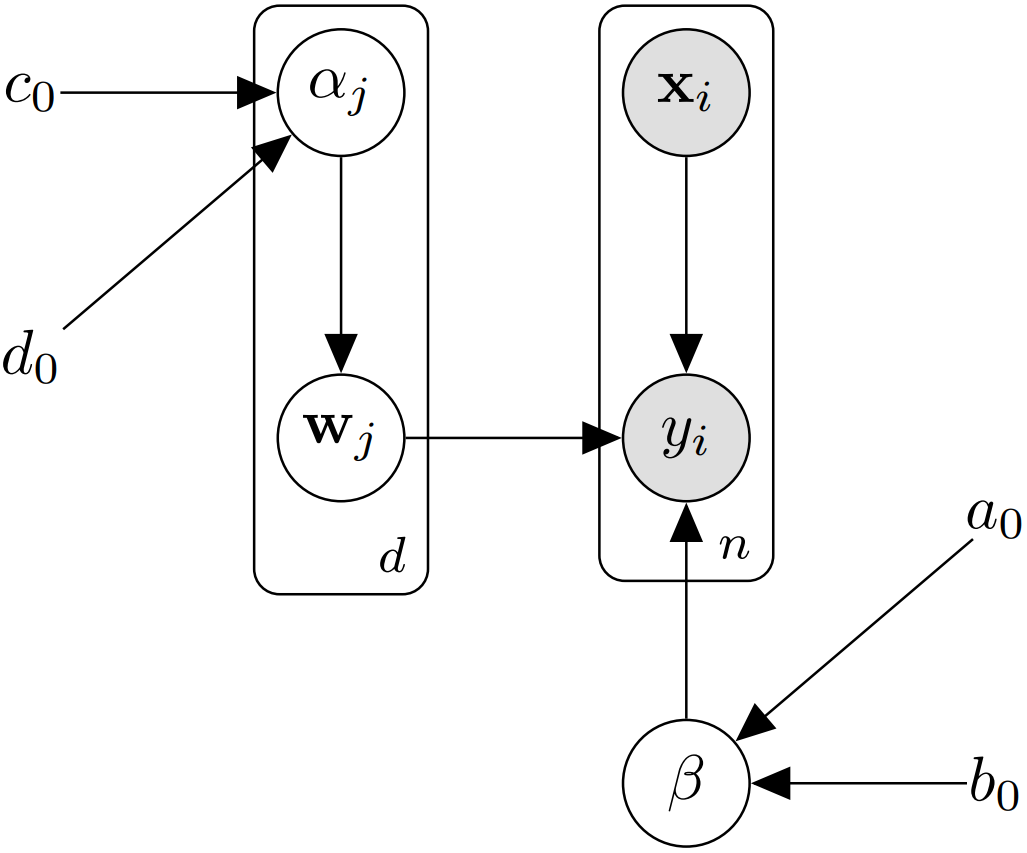
\includegraphics[width=0.5\textwidth]{bn_network.png} 
        \caption{Plate diagram of the regression model with ARD prior. Variables $x_i$ , and $y_i$ are observed; We are interested in the posterior distribution of parameters $w$, $\alpha$ and $\beta$. The constants $a_0$ , $b_0$, $c_0$ , and $d_0$ are user-defined hyperparameters}
        \label{fig:diagram}
    \end{figure}

    The components so far can be represented as a Bayesian network, illustrated in Figure \ref{fig:diagram}. The posterior can be conveniently deducted from the diagram to be
    \begin{align*}
        P(w,\alpha,\beta|y,x) \propto \prodlim{1}{n}P(y_i|w,x_i,\beta)\prodlim[j]{1}{d}\enclb{P(w_j|\alpha_j)P(\alpha_j)}P(\beta). \numberthis\label{eq:posterior}
    \end{align*}

\section{Gibbs sampling and conjugate priors}
    Gibbs sampling will be used to approximate the optimal ARD regression model parameters. Gibbs sampler requires the full conditional distributions for the model parameters; $P(w|y,x,\alpha,\beta)$, $P(\alpha|y,x,w,\beta)$, $P(\beta|y,x,w,\alpha)$, where $\alpha=(\alpha_1,\ldots,\alpha_d)$. 

    \subsection{Deriving conjugate prior for \texorpdfstring{$w$}{}}
        \begin{align*}
            %
            & P(w|y,x,\alpha,\beta) \propto \prodlim{1}{n}P(y_i|w,x_i,\beta) \prodlim[j]{1}{d}P(w_j|\alpha_j) \\ 
            & = N(y_i|X^Tw) \prodlim[j]{1}{d} N(w_j|0,(\sqrt{\alpha_j})^{-1})\\ 
            & \propto \exp\enclp{-\frac{1}{2}\beta(y-X^Tw)^T(y-X^Tw)} \prodlim[j]{1}{d} \exp\enclp{-\frac{1}{2} w^2(\sqrt{\alpha_j})^2} \\
            & = \exp\enclp{-\frac{1}{2}\beta(y-X^Tw)^T(y-X^Tw) - \frac{1}{2} \sumlim[j]{1}{d} w^2 \alpha} \\ 
            & = \exp\enclp{-\frac{1}{2}\beta(y-X^Tw)^T(y-X^Tw) - \frac{1}{2} w^T D w}
        \end{align*}
        where $D$ is a $d \times d$ diagonal matrix with the values $\alpha_1, \alpha_2, \ldots, \alpha_d$   
    
        Completing the square seems reasonable at this point, now the goal is to complete the square, that is get the exponent in the form $\frac{1}{2}w^TAw+k^Tw$. For convenience we will take the logarithm to remove the base exponential:
        \begin{align*}
                %
                \Rightarrow \log P(w|y,x,\alpha,\beta) &\propto -\frac{1}{2}\beta \enclp{y^Ty - y^TX^Tw - w^TXy + w^TXX^Tw} - \frac{1}{2} w^T D w \\ 
                &\propto -\frac{1}{2} \enclb{-2\beta y^TX^Tw + \beta w^TXX^Tw} - \frac{1}{2} w^T D w \\ 
                &= \beta y^TX^Tw -\frac{1}{2} \beta w^TXX^Tw - \frac{1}{2} w^T D w \\ 
                &= -\frac{1}{2} \enclb{w^T\beta XX^Tw + w^T D w} + \beta y^TX^Tw \\
                &= -\frac{1}{2} w^T \undertext{\enclp{\beta XX^T + D}}{$=A$} w + \undertext{\beta y^TX^T}{$=k^T$}w
        \end{align*}
    
        Then by completing the square we obtain the parameters $S$ (covariance) and $m$ (mean) for a Multivariate Gaussian that is proportional to $P(w|y,x,\alpha,\beta)$:
        \begin{align*}
            S &= A^{-1} = \enclp{\beta XX^T + D}^{-1} \\ 
            m &= A^{-1}k = S \beta Xy\\
            &\dunderline{\Rightarrow P(w|y,x,\beta) \propto \mathcal{N}(w|m,S)} \numberthis\label{eq:wconjugate}
        \end{align*}

    \subsection{Deriving conjugate prior for \texorpdfstring{$\alpha$}{}}
        \begin{align*}
            %
            P(\alpha|y,x,w,\beta) &\propto \prodlim[j]{1}{d}P(w_j|\alpha_j)P(\alpha_j) \\ 
            &= \prodlim[j]{1}{d} N(w_j|0,\alpha^{-1}) \opGamma(a_j|c_0,d_0) \\ 
            &\propto \prodlim[j]{1}{d} \frac{1}{\sqrt{\alpha_j^-1}} \exp\enclp{-\frac{1}{2} \enclb{\frac{w_j}{\sqrt{\alpha}^{-1}}}^2}\alpha_j^{c_0-1} \exp\enclp{-d_0\alpha_j} \\ 
            &= \prodlim[j]{1}{d} \exp\enclp{-\frac{w_j^2}{2}\alpha_j - d_0\alpha_j}\alpha_j^{c_0-1+1/2} \\ 
            &= \prodlim[j]{1}{d} \exp\enclp{-\alpha_j\enclp{\frac{w_j^2}{2}+d_0}}\alpha_j^{c_0-1+1/2} \\ 
            &\propto \dunderline{\prodlim[j]{1}{d} \opGamma(\alpha_j|c_0+\frac{1}{2},\frac{w_j^2}{2}+d_0)} \numberthis\label{eq:alphaconjugate}
        \end{align*}

        To sample an $\alpha_j$ from the distribution we simply sample from $\opGamma(\alpha_j|c_0-\frac{1}{2},\frac{w_j^2}{2}+d_0)$.

    \subsection{Deriving conjugate prior for \texorpdfstring{$\beta$}{}}
        \begin{align*}
            %
            P(\beta|y,x,w,\alpha) &\propto P(\beta)\prodlim{1}{n}P(y_i|w,x_i,\beta)\\ 
            &= \opGamma(\beta|a_0, b_0) \prodlim{1}{n}N(y_i|w^Tx_i,\sqrt{\beta^{-1}})\\
            &= \beta^{a_0-1} \exp\enclp{-b_0\beta} \prodlim{1}{n} \frac{1}{\sqrt{\beta^{-1}}} \exp\enclp{-\frac{1}{2}\enclp{\frac{y_i-w^Tx_i}{\sqrt{\beta^{-1}}}}^2} \\ 
            &= \beta^{a_0-1} \exp\enclp{-b_0\beta} \enclp{\beta^{1/2}}^n \exp\enclp{-\frac{1}{2}\sumlim{1}{n}\beta(y_i-w^Tx_i)^2} \\ 
            &= \beta^{a_0-1}\beta^{n/2}\exp\enclp{-b_0\beta-\frac{\beta}{2}\sumlim{1}{n}(y_i-w^Tx_i)^2} \\ 
            &= \beta^{a_0-1+n/2} \exp\enclp{-\beta\enclp{b_0+\frac{1}{2}\sumlim{1}{n}(y_i-w^Tx_i)^2}} \\ 
            & \dunderline{\propto \opGamma(\beta|a_0+n/2, b_0+\frac{1}{2}\sumlim{1}{n}(y_i-w^Tx_i)^2)} \numberthis\label{eq:betaconjugate}
        \end{align*}

    \subsection{Implementation}
        Only polynomial kernel lololol xD xD xD

\section{Simulation study}
    To test the regression using ARD against the counterpart which does not use ARD we simulate some datasets to test on. The generated data will be generated using multivariate polynomials, as the implementation of the regression models are only capable of using polynomial features. 

    \subsection{The datasets}
        The simulated data will be generated from $6$ polynomial functions:
        \begin{align}
            f_1(x,y)&=-4x+20y^2x+69 \label{eq:f1}\\
            f_2(x,y)&=69x+69y-420 \label{eq:f2}\\
            f_3(x,y)&=x^2-2y^2 \label{eq:f3}\\
            f_4(x,y)&=xy-x^2+y^2-420 \label{eq:f4}\\
            f_5(x,y)&=-x^3+42x^2-20x-y^3+42y^2-20y+69 \label{eq:f5}\\
            f_6(x,y)&=2x^3-y^3-3xy^2+3x^2y+x^3-3yx+69 \label{eq:f6}
        \end{align}

        The method of generating the data is simple. For each function $f_i$ do:
        \begin{enumerate}
            \item Randomly generate some data $X$ from the domain of $f_i$
            \item Obtain response values $y$ by inputting $X$ into $f_i$
            \item Offset each value of $y$ with gaussian noise (same noise distribution for all elements in $y$)
        \end{enumerate}

        The domain sampling distribution and noise distribution with respect for each function are as follows:
        \begin{table}[H]
            \centering
            \caption{Note that the domain distributions are univariate even though the functions are multivariate. Values from the domain distributions are simply sampled repeatedly for each variable, in this case $x$ and $y$.}
            \begin{tabular}{crr}
                \toprule
                function & domain distribution & noise distribution \\ 
                \midrule
                $f_1(x,y)$ & $\operatorname{Exp}(\text{rate}=5)$    & $N(0,22)$  \\
                $f_2(x,y)$ & $N(\text{mean}=69, \text{std}=4)$      & $N(0,420)$ \\
                $f_3(x,y)$ & $\operatorname{Unif}(\min=-2,\max=20)$ & $N(0,69)$  \\ 
                $f_4(x,y)$ & $N(\text{mean}=0, \text{std}=8)$       & $N(0,22)$  \\
                $f_5(x,y)$ & $\operatorname{Exp}(\text{rate}=5)$    & $N(0,420)$ \\
                $f_6(x,y)$ & $\operatorname{Unif}(\min=-6,\max=6)$  & $N(0,69)$  \\
                \bottomrule
            \end{tabular}
        \end{table}

        Then generating $128$ data samples for each function produces the following plots:
        \begin{figure}[H]
            \centering
            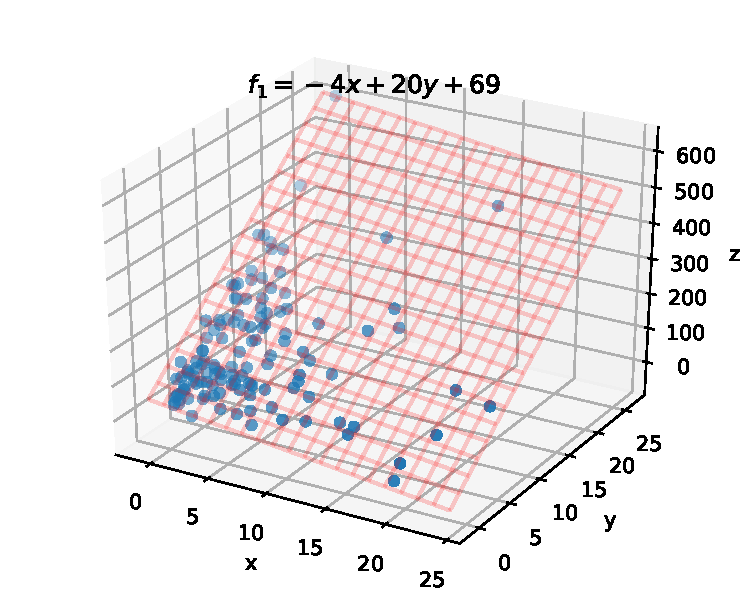
\includegraphics[width=0.49\textwidth]{f_1.pdf}
            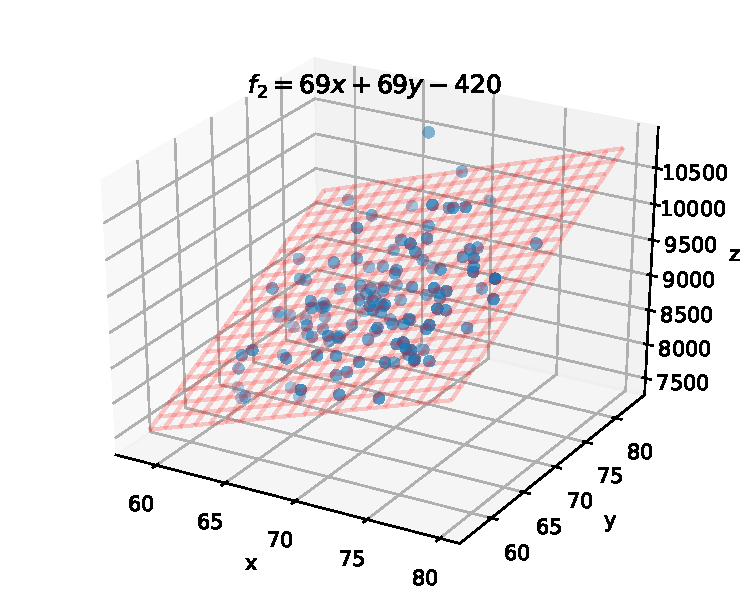
\includegraphics[width=0.49\textwidth]{f_2.pdf}
            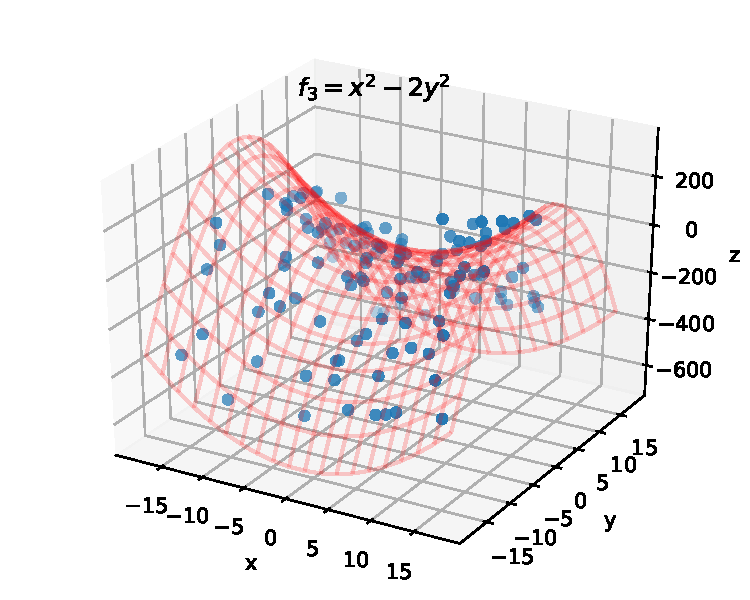
\includegraphics[width=0.49\textwidth]{f_3.pdf}
            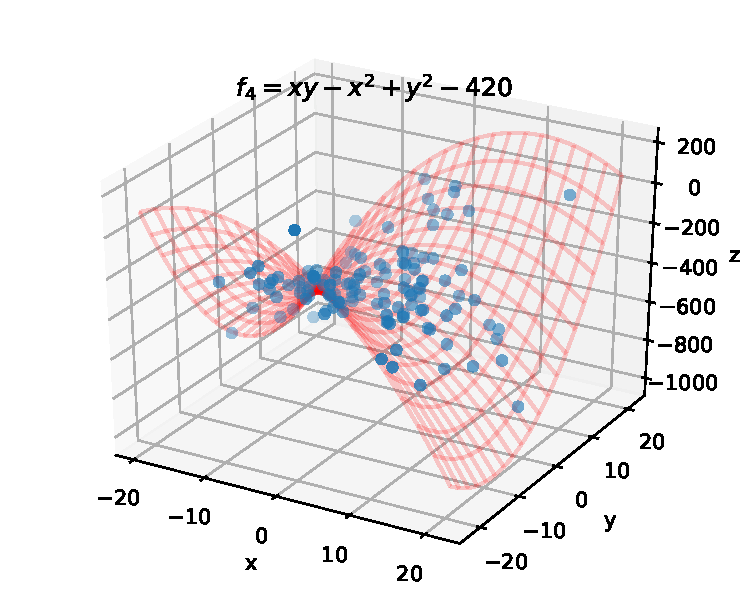
\includegraphics[width=0.49\textwidth]{f_4.pdf}
            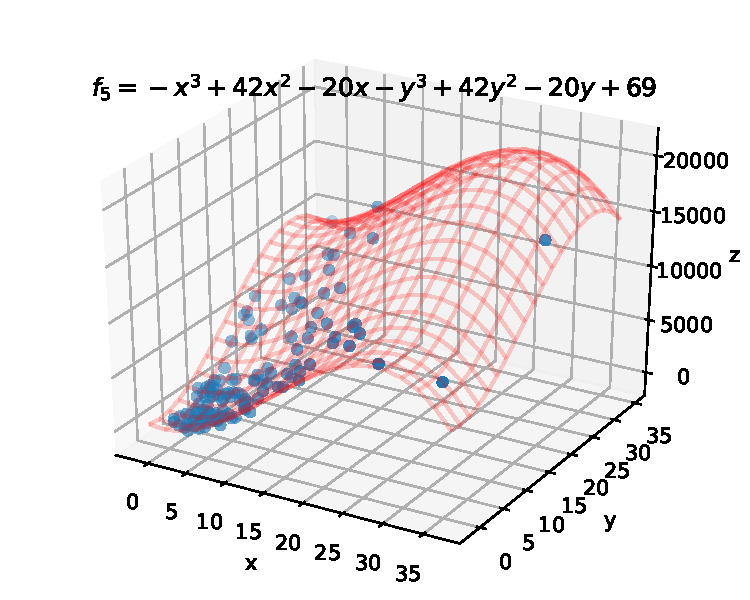
\includegraphics[width=0.49\textwidth]{f_5.pdf}
            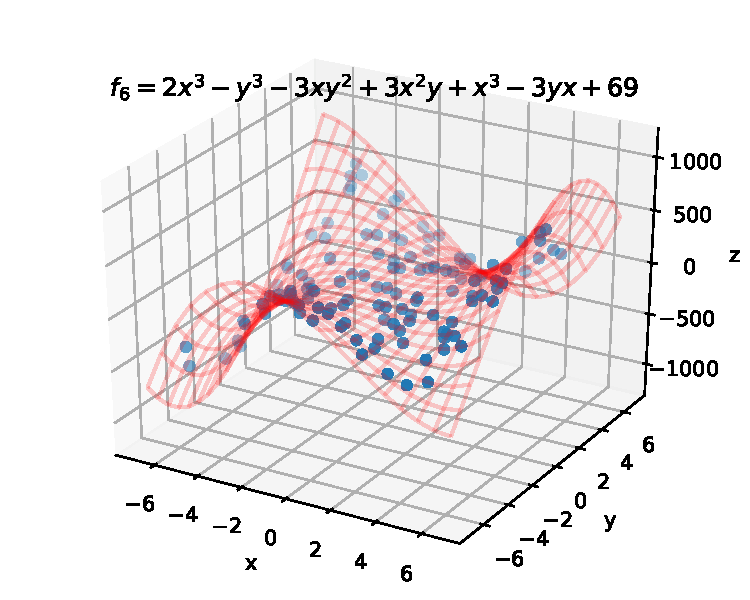
\includegraphics[width=0.49\textwidth]{f_6.pdf}
            \caption{}
        \end{figure}
    
    \subsection{Regression on the generated data}
        We fit regression models using ARD and without ARD to assess the differences in performance. We use the mean squared error between the true and estimated parameters. To assess the models' performances under presence of irrelevant features, we simply a add few extra features to the data that does not affect the response variables.
        \begin{table}[H]
            \centering
            \caption{"noise\_features" column indicates number of added irrelevant features to the data. The degree column indicates which degree the polynomial regression was done in.}
            \begin{tabular}{llrrrr}
                \toprule
                  &       &  degree &  ARD MAE &  Regular MAE &  Regular over ARD \\
                noise features & function &         &          &              &                   \\
                \midrule
                0 & $f_1$ &       1 &    18.27 &       109.55 &              6.00 \\
                & $f_2$ &       1 &   336.33 &      8914.98 &             26.51 \\
                & $f_3$ &       2 &    48.91 &        48.86 &              1.00 \\
                & $f_4$ &       2 &    17.65 &       249.43 &             14.13 \\
                & $f_5$ &       3 &   314.27 &      2326.37 &              7.40 \\
                & $f_6$ &       3 &    49.44 &        59.51 &              1.20 \\
                \midrule
                1 & $f_1$ &       1 &    18.57 &        82.77 &              4.46 \\
                & $f_2$ &       1 &   347.24 &      8848.73 &             25.48 \\
                & $f_3$ &       2 &    54.41 &        55.03 &              1.01 \\
                & $f_4$ &       2 &    15.18 &       232.57 &             15.32 \\
                & $f_5$ &       3 &   322.23 &      1954.00 &              6.06 \\
                & $f_6$ &       3 &    53.24 &        56.67 &              1.06 \\
                \midrule
                2 & $f_1$ &       1 &    16.91 &        72.16 &              4.27 \\
                & $f_2$ &       1 &   312.72 &      8816.07 &             28.19 \\
                & $f_3$ &       2 &    51.41 &        51.67 &              1.01 \\
                & $f_4$ &       2 &    16.46 &       218.45 &             13.27 \\
                & $f_5$ &       3 &   297.41 &      1975.98 &              6.64 \\
                & $f_6$ &       3 &    54.04 &        59.68 &              1.10 \\
                \midrule
                3 & $f_1$ &       1 &    16.69 &        69.08 &              4.14 \\
                & $f_2$ &       1 &   325.36 &      8756.69 &             26.91 \\
                & $f_3$ &       2 &    55.46 &        55.37 &              1.00 \\
                & $f_4$ &       2 &    17.47 &       177.05 &             10.13 \\
                & $f_5$ &       3 &   335.03 &      2139.92 &              6.39 \\
                & $f_6$ &       3 &    54.70 &        59.95 &              1.10 \\
                \bottomrule
            \end{tabular}
        \end{table}

    \appendix
    
    % \bibliographystyle{apalike}
    % \bibliographystyle{ieeetran}
    % \bibliography{citations}
    
    \end{document}
    